% !TeX root = ../main.tex
% Add the above to each chapter to make compiling the PDF easier in some editors.

\chapter{Methodology}\label{chapter:methodology}
This chapter details our approach to developing and evaluating visualization interfaces for perception modification tasks in teleoperation. Our methodology addresses three key aspects: interface design, implementation of the Integrated View approach, and performance optimization.

The development process follows user-centered design principles, focusing on meeting the requirements established in Section 2.7.1. We implement two distinct interfaces - the Separate View and Integrated View - to compare their effectiveness in supporting perception modification tasks. Both interfaces are built on the ToD Visual 2.0 framework, ensuring consistent baseline functionality while enabling fair comparison of their unique visualization approaches.
\section{Interface Design}
Before talking about the implementation, we first need to discuss the interface design.
We need to design the two interfaces, we compare such that they are good fits to our requirements,
they are implementable in a reasonable amount of time, and also they need to cover same features
to not bias the study results towards one interface with more features. We begin by discussing the Separate View interface.



\subsection{Separate View}
The Separate View approach presents environmental perception data through two distinct windows. The first window provides the camera feed, supporting multiple camera outputs simultaneously. The second window offers a comprehensive 3D visualization of the vehicle's perception data and environmental model \cite{Kettwich}.

The 3D visualization window integrates several key components developed by El Alami \cite{yassinethesis}: The features are shown in Table \ref{table:interface_features}.

This dual-window approach allows operators to directly compare raw sensor data with the vehicle's perception outputs, facilitating the identification of potential perception errors or misclassifications \cite{Georg}. While the implementation details of these visualization features are covered in El Alami's work \cite{yassinethesis}, they form essential components of both our interface approaches and serve as the foundation for our comparative analysis.

\subsection{Integrated View}
To implement the Integrated View approach, which combines raw sensor data and perception outputs in a unified visualization, we selected Depth Completion as the primary method for creating a coherent 3D representation. This approach allows us to generate dense depth maps from sparse LiDAR data, which can then be used to create point clouds onto which camera images are projected.

The camera configuration is crucial in this setup, as it is the primary visual information source. Research has shown that field of view (FOV) significantly impacts teleoperation performance. Studies indicate that a 200° FOV enables 40\% higher average speeds compared to 40° FOV, and a 120° FOV reduces stopped time by half compared to 40° FOV \cite{fovConsiderations}. However, wider FOVs can increase motion sickness and scene distortion. A horizontal FOV between 120 and 200 degrees provides optimal performance for teleoperation tasks \cite{fovConsiderations}. We selected a 120-degree FOV to balance performance requirements with information density and cognitive load considerations.

For video quality, we opted for 1280x720 resolution at 30 frames per second. This configuration requires 1.5 to 3 Mbit/s upstream bandwidth \cite{vdocipher2024bandwidth}, which aligns with the average network capabilities in Germany. As the camera stream represents the primary bandwidth constraint, this resolution provides the highest quality possible while maintaining reliable transmission.

The completed point cloud is a base layer for additional perception data visualization. We overlay this with the perception information from the Separate View shown in the Table \ref{table:interface_features}.

The detailed implementation of these components and the depth completion approach are discussed in Section \ref{section:integratedviewimplementation}.

\begin{table}[h!]
    \centering
    \begin{tabular}{@{}p{3cm}p{5.3cm}p{5.3cm}@{}}
    \toprule
    \textbf{Feature Category} & \textbf{Separate View} & \textbf{Integrated View} \\
    \midrule
    Visualization \par Approach & Two distinct windows: one for camera feed and another for 3D visualization of perception data. & Unified visualization combining raw sensor data and perception outputs into a single window. \\
    \midrule
    Camera Feed & Supports multiple camera outputs simultaneously in a dedicated window. & Camera images are projected onto a dense point cloud generated through depth completion. \\
    \midrule
    Point Cloud Data & Displayed in a separate 3D visualization window. & Generated using depth completion from sparse LiDAR data and overlaid with camera projections. \\
    \midrule
    Object Detection & Color-coded bounding boxes for object detection and classification in 3D visualization. & Same as Separate View. \\
    \midrule
    Lanelet Map & Lanelet map visualization with regulatory elements in the 3D visualization window. & Same as Separate View. \\
    \midrule
    Trajectory \par Visualization & Planned trajectory visualization for the ego vehicle and prediction trajectories for other traffic participants displayed in 3D visualization. & Same as Separate View. \\
    \bottomrule
    \end{tabular}
    \caption{Comparison of Features Between Separate View and Integrated View Interfaces}
    \label{table:interface_features}
    \end{table}


\section{Integrated View Implementation}\label{section:integratedviewimplementation}

The Integrated View implementation consists of several key components that work together to create a unified visualization of environmental perception data. This section details the technical implementation of each component, starting with the fundamental camera-to-point-cloud projection and continuing through depth completion, rendering, and the complete system integration.

The pipeline for generating the integration starts with estimating a depth map of the environment using a depth completion model, creating a point cloud out of this depth map, and then projecting the camera image onto this point cloud to have a realistic rendering of the environment in the end that can be seen in Figure \ref{fig:depth_completion_result}. The following sections detail the implementation of each step in this pipeline.

\subsection{Camera to Point Cloud Projection}

\begin{figure}
    \centering
    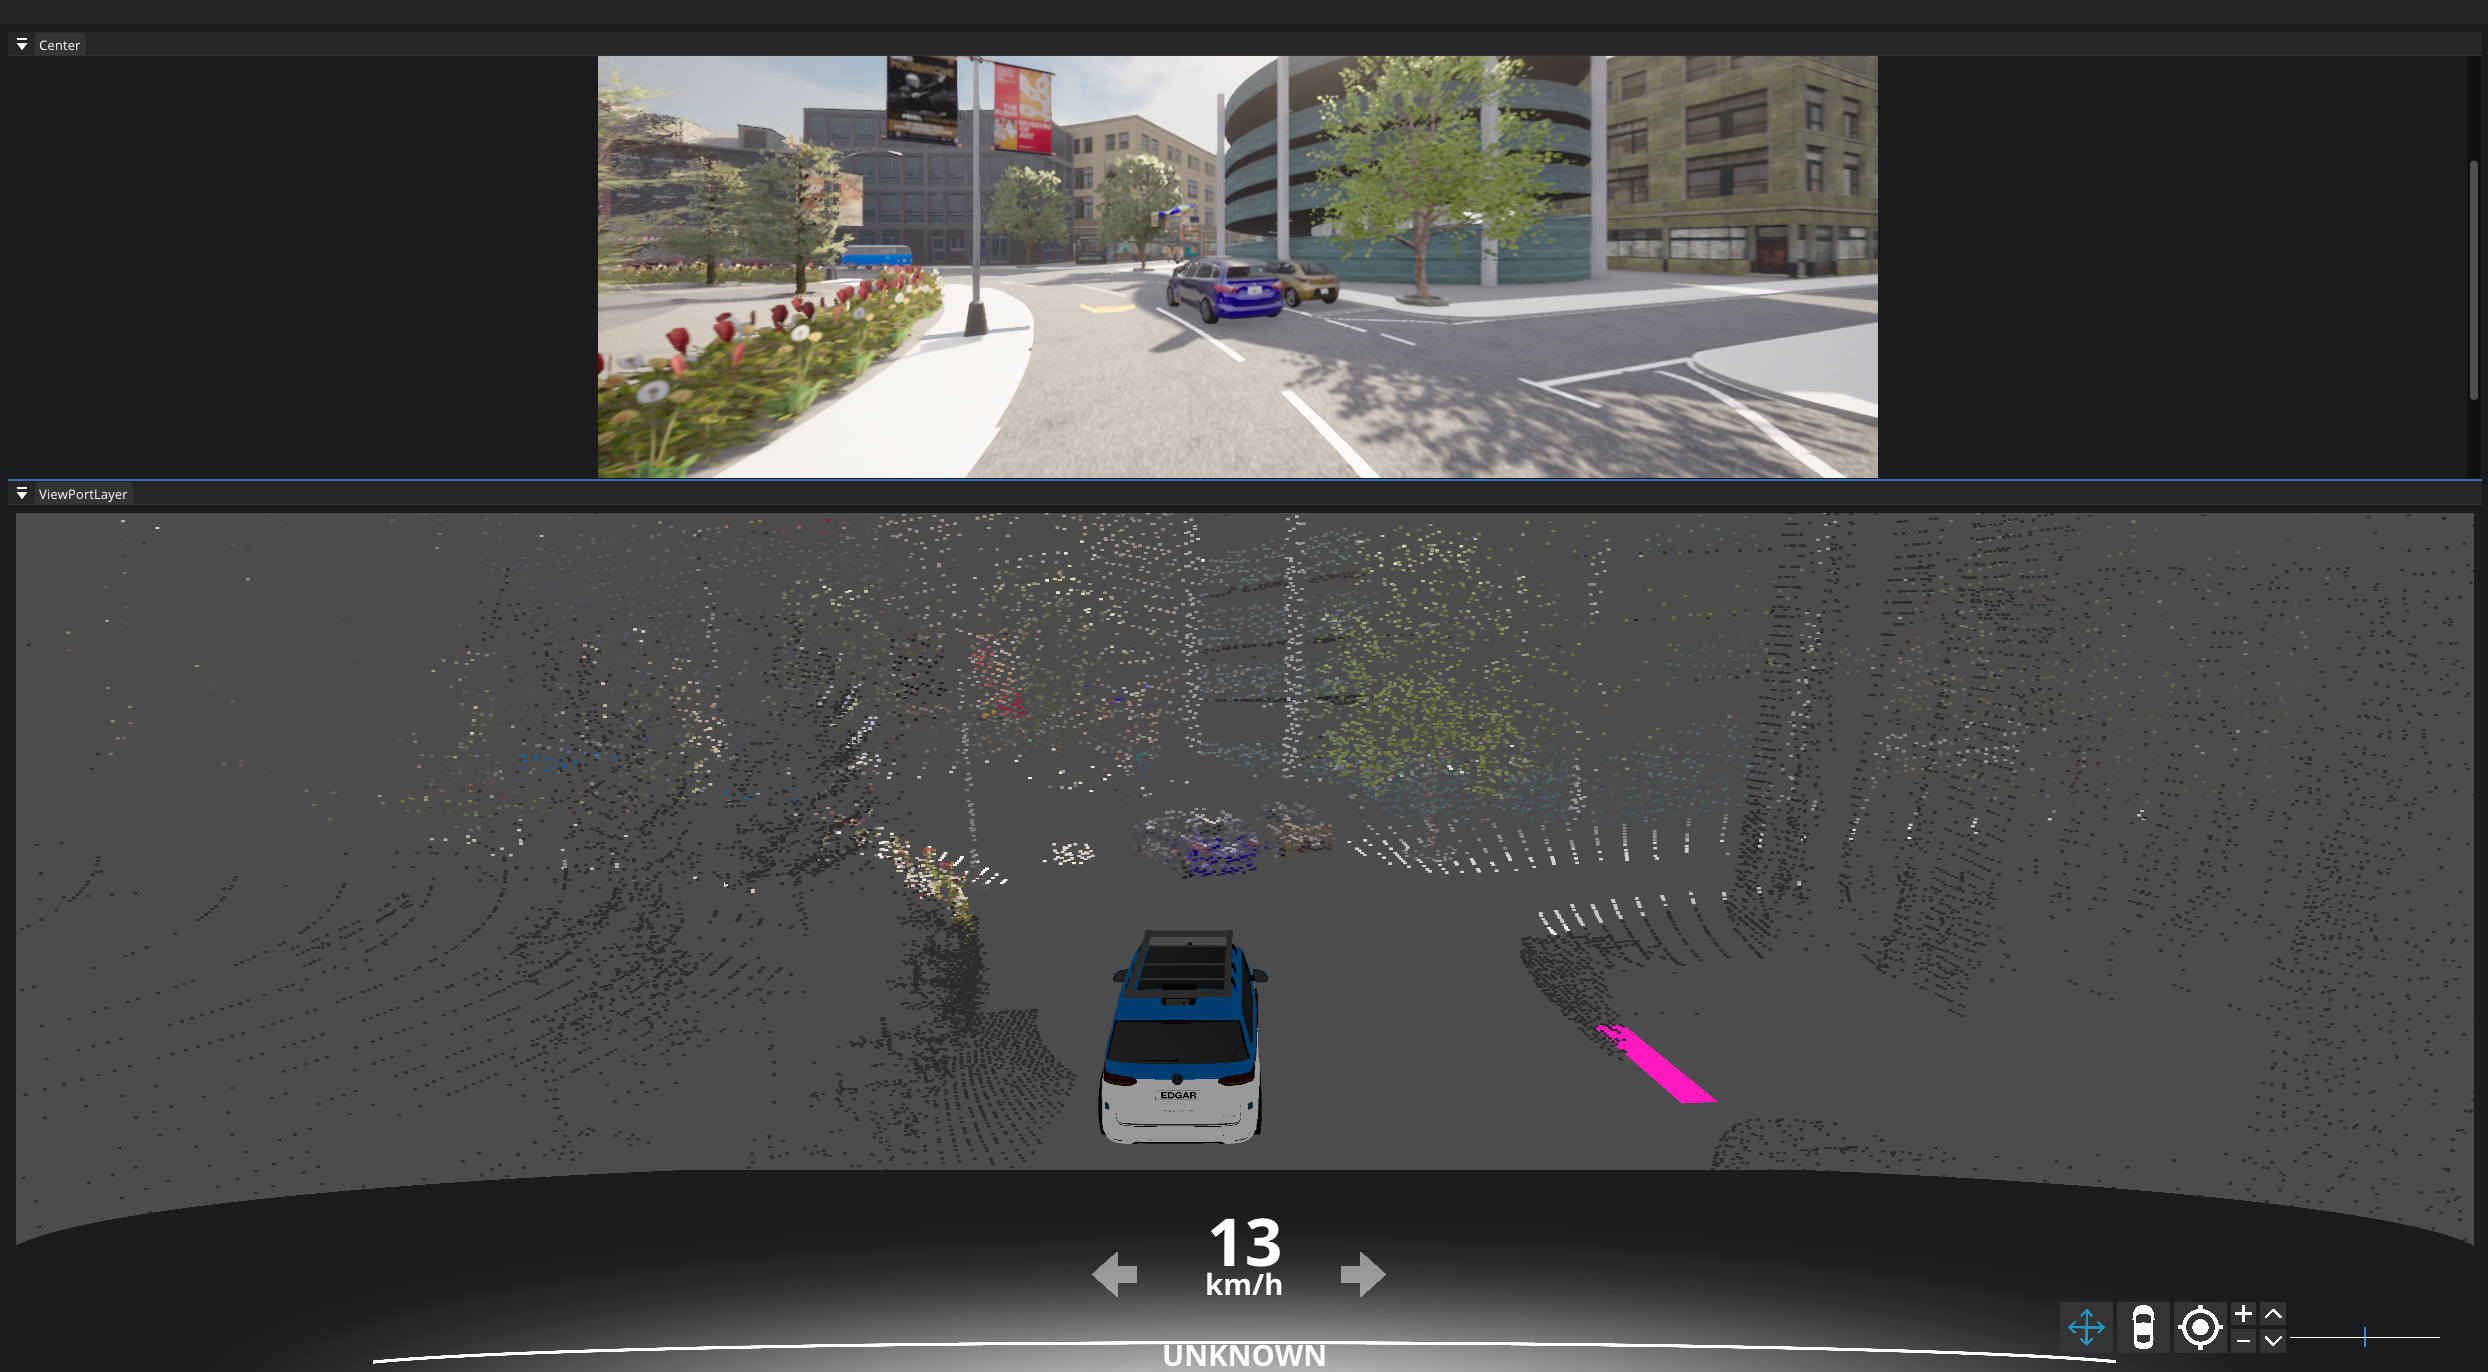
\includegraphics[width=\textwidth, trim=0 150pt 0 50pt, clip]{figures/pc.png}
    \caption{Lidar point cloud from the simulation colored by camera projection}
    \label{fig:camera_projection}
\end{figure}

The first step in creating our Integrated View is establishing an accurate projection between the camera image space and the 3D LiDAR point cloud. This process involves several mathematical transformations to align the different coordinate systems and project 3D points onto the 2D image plane.

\subsubsection{Coordinate System Transformations}

To project a 3D point from the LiDAR coordinate system to the camera image plane, we perform the following sequence of transformations:
\begin{enumerate}
    \item Transform the point from LiDAR coordinates to camera coordinates using extrinsic parameters.
    \item Project the transformed point onto the camera's image plane using intrinsic parameters.
    \item Apply the color information from the projected pixel back to the 3D point.
\end{enumerate}

The mathematical representation of this process can be expressed as:

\[
p_{\text{cam}} = T_{\text{cam}}^{\text{lidar}} \cdot p_{\text{lidar}}
\]

where \( T_{\text{cam}}^{\text{lidar}} \) is the transformation matrix from LiDAR to camera coordinates, and \( p_{\text{lidar}} \) is a point in LiDAR coordinates represented in homogeneous form:

\[
p_{\text{lidar}} = \begin{bmatrix} x \\ y \\ z \\ 1 \end{bmatrix}
\]

\subsubsection{Camera Projection Model}

The projection of 3D points onto the image plane follows the pinhole camera model. Given the camera's intrinsic matrix \( K \):

\[
K = \begin{bmatrix}
f_x & 0 & c_x \\
0 & f_y & c_y \\
0 & 0 & 1
\end{bmatrix}
\]

The projection equation becomes:

\[
\begin{bmatrix} u \\ v \\ 1 \end{bmatrix} = K \begin{bmatrix} R | t \end{bmatrix} \begin{bmatrix} X \\ Y \\ Z \\ 1 \end{bmatrix}
\]

where:
\begin{itemize}
    \item \( (u,v) \) are the pixel coordinates in the image,
    \item \( (X,Y,Z) \) are the 3D point coordinates in camera space,
    \item \( R \) is the rotation matrix,
    \item \( t \) is the translation vector.
\end{itemize}

\subsubsection{Color Assignment}

After projection, we determine the color information for each 3D point by sampling the corresponding pixel in the camera image. To handle cases where multiple 3D points project to the same pixel, we implement a depth-based selection strategy:

\[
\text{color}(p) =
\begin{cases}
I(u,v) & \text{if } z_{\min} \leq z \leq z_{\max} \\
0 & \text{otherwise}
\end{cases}
\]

where:
\begin{itemize}
    \item \( I(u,v) \) is the image color at pixel coordinates \( (u,v) \),
    \item \( z_{\min} \) and \( z_{\max} \) define the valid depth range.
\end{itemize}

This projection process forms the foundation for our Integrated View,
enabling the combination of LiDAR point cloud data with camera imagery as seen in the figure \ref{fig:camera_projection}.
We see it as a critical step in creating a coherent 3D representation of the vehicle's environment.
Thus we also employed this method in the Separate View to color the raw point cloud
coming from the Lidar sensors.

In the next section we discuss how to populate the point cloud from a depth map. What's good about this
projection method is it being input agnostic, meaning it can be used either with a depth map point cloud,
or a raw point cloud from a Lidar sensor without any changes.

\subsection{Depth Cloud Rendering}

\begin{figure}
    \centering
    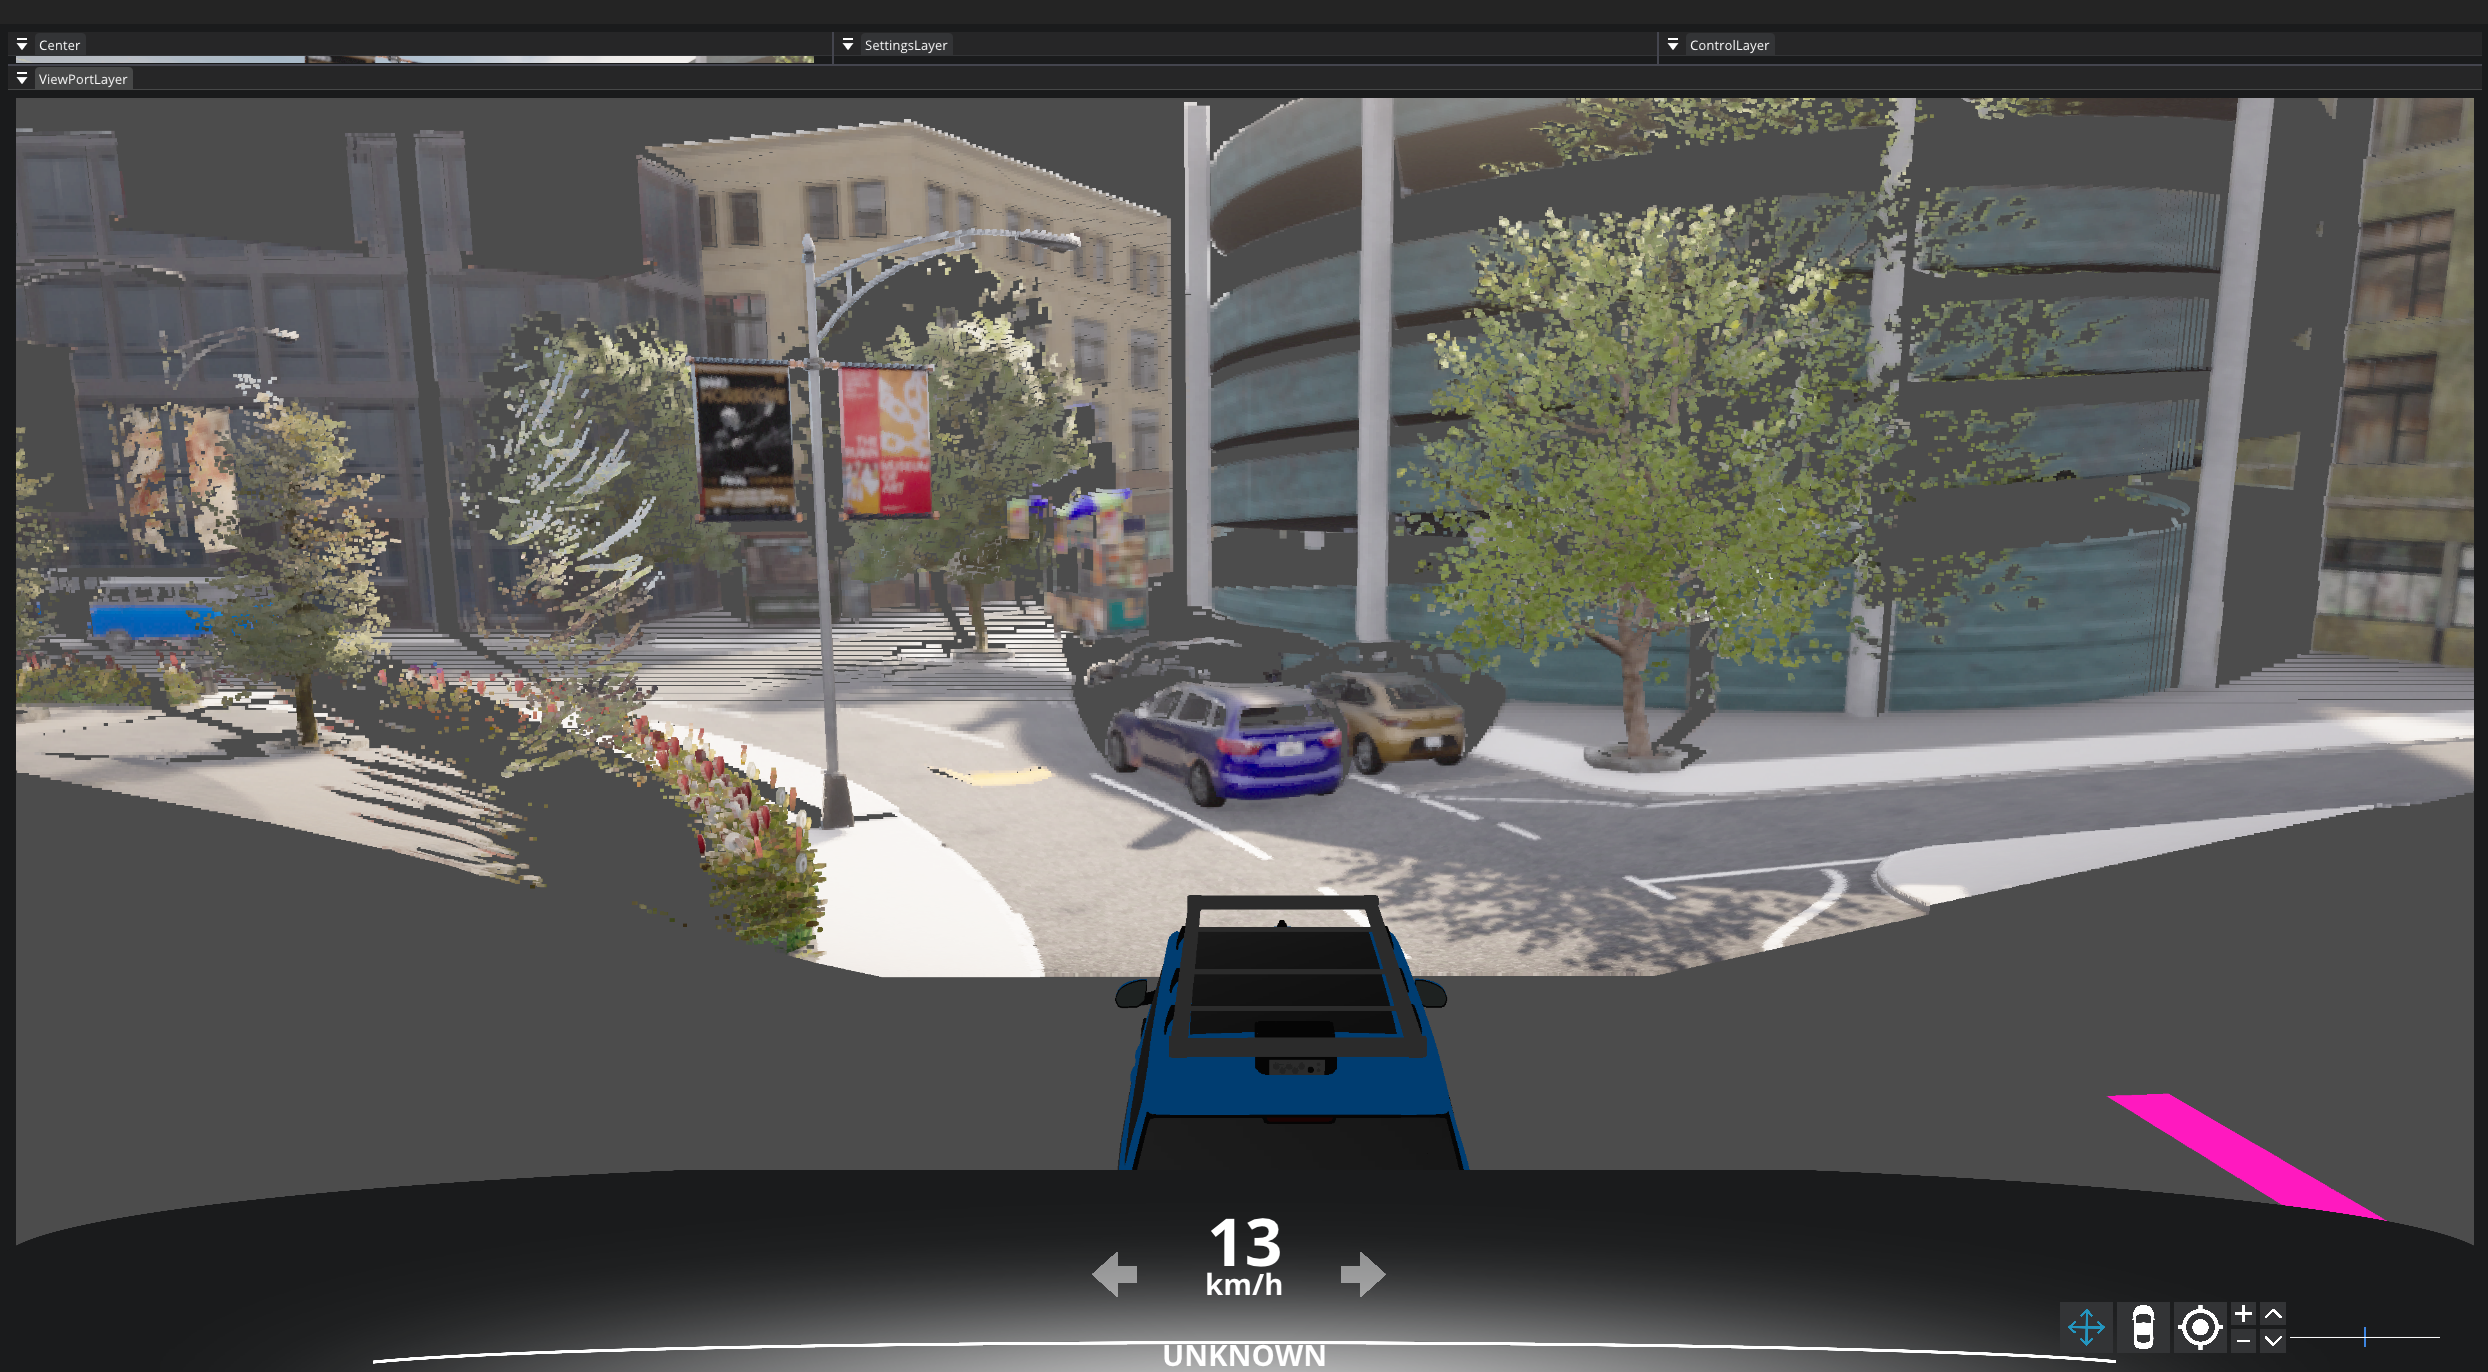
\includegraphics[width=\textwidth, trim=0 150pt 0 50pt, clip]{figures/gt.png}
    \caption{Depth cloud rendering from a the ground truth depth map}
    \label{fig:depth_cloud}
\end{figure}

Depth cloud rendering is a crucial step in creating the Integrated View, as it involves generating a 3D point cloud from a depth image. This process allows for the visualization of environmental data in a spatially accurate and intuitive format. For this implementation, we utilized the depth camera provided by the CARLA simulation environment. While CARLA's depth camera provides precise depth information in simulation as it can be seen from figure \ref{fig:depth_cloud}. It is important to note that such sensors do not exist in real life. Real-world depth cameras, such as stereo cameras or LiDAR-based systems, have significant limitations, including reduced accuracy under poor lighting conditions or sparse data points.

\subsubsection{Depth Camera in CARLA}

In CARLA, the depth camera generates a depth image where each pixel encodes the distance of a point in the scene from the camera plane. The depth values are stored as floating-point numbers, representing distances in meters. This simulated sensor provides an idealized output without noise or inaccuracies, making it suitable for testing visualization techniques but not representative of real-world conditions.

The transformation from a depth image to a 3D point cloud involves converting each pixel into its corresponding 3D coordinates in the camera coordinate system. This is achieved using the intrinsic parameters of the camera, which include focal lengths (\(f_x\), \(f_y\)) and principal point offsets (\(c_x\), \(c_y\)).

\subsubsection{Mathematical Transformation}

To convert a depth image into a 3D point cloud, we use the following equations:

1. For each pixel \((u, v)\) in the image:
   \[
   X = \frac{(u - c_x) \cdot d}{f_x}, \quad
   Y = \frac{(v - c_y) \cdot d}{f_y}, \quad
   Z = d
   \]
   where:
   \begin{itemize}
    \item[--] \(X, Y, Z\) are the 3D coordinates of the point in the camera coordinate system,
    \item[--] \(u, v\) are the pixel coordinates,
    \item[--] \(d\) is the depth value at pixel \((u, v)\),
    \item[--] \(f_x, f_y\) are the focal lengths of the camera,
    \item[--] \(c_x, c_y\) are the principal point offsets.
   \end{itemize}

2. Each calculated 3D point is then represented as:
   \[
   p_{\text{camera}} = \begin{bmatrix} X \\ Y \\ Z \\ 1 \end{bmatrix}
   \]

3. To integrate color information into the point cloud:
   - For each pixel \((u, v)\), retrieve its RGB values from the corresponding color image.
   - Assign these RGB values to the 3D point.

\subsubsection{Implementation Considerations}

The implementation involves iterating over each pixel in the depth image and applying the above transformation to compute its 3D coordinates. Special care is taken to handle invalid or out-of-range depth values:
- Pixels with non-finite or zero depth values are ignored.
- Depth values exceeding a predefined range (e.g., maximum sensor range) are discarded.

The final step combines these 3D points with their corresponding color information to generate a complete colored point cloud.

\subsubsection{Limitations of Real-World Depth Cameras}

Unlike CARLA's idealized depth camera, real-world depth cameras face several challenges, as summarized in Table~\ref{table:depth_camera_limitations}.

\begin{table}[h!]
\centering
\begin{tabular}{@{}p{4cm}p{10cm}@{}}
\toprule
\textbf{Limitation} & \textbf{Description} \\
\midrule
Noise and Accuracy & Stereo cameras rely on disparity calculations and can struggle with low-texture regions or poor lighting conditions. \\
\midrule
Sparse Data & LiDAR sensors provide high-accuracy distance measurements but produce sparse point clouds that require interpolation or fusion with other sensors. \\
\midrule
Field of View & Real-world cameras often have limited fields of view compared to simulated sensors. \\
\bottomrule
\end{tabular}
\caption{Limitations of Real-World Depth Cameras}
\label{table:depth_camera_limitations}
\end{table}

These limitations highlight why CARLA's simulated depth camera is used for prototyping and testing visualization approaches but the approach cannot be used in real-world conditions.
For this reason we implemented our neural networks based depth completion method to generate a dense point cloud from sparse LiDAR data, which is explained in the next section.

Depth cloud rendering forms a foundational part of our Integrated View implementation by enabling accurate spatial visualization of environmental data. The resulting colored point cloud serves as a base layer for integrating additional perception outputs such as object detections and lanelet maps.
\subsection{Depth Completion}
As mentioned in the last section, we must rely on something other than depth cameras for long distances. The LiDAR sensors provide accurate depth measurements, but their sparse nature limits our ability to create a comprehensive 3D visualization of the environment.
Depth completion addresses this limitation by converting sparse depth data into dense depth maps by fusing LiDAR and camera data. This approach is particularly relevant for our Integrated View implementation, as it enables the creation of detailed, spatially accurate scene reconstructions.

For our implementation, we selected the DySPN (Dynamic Spatial Propagation Network) architecture \cite{dyspn}, which introduces a non-linear propagation model for depth completion. Figure \ref{fig:dyspn_architecture} shows that the network employs a ResNet34-UNet backbone that generates an initial depth map, affinity matrix, and a series of spatial and sequential attention maps. The key innovation of DySPN lies in its dynamic approach to spatial propagation - unlike previous methods \cite{cheng2020cspn} that use fixed affinity matrices, DySPN adaptively adjusts the affinity weights during propagation through attention mechanisms.

\begin{figure}
    \centering
    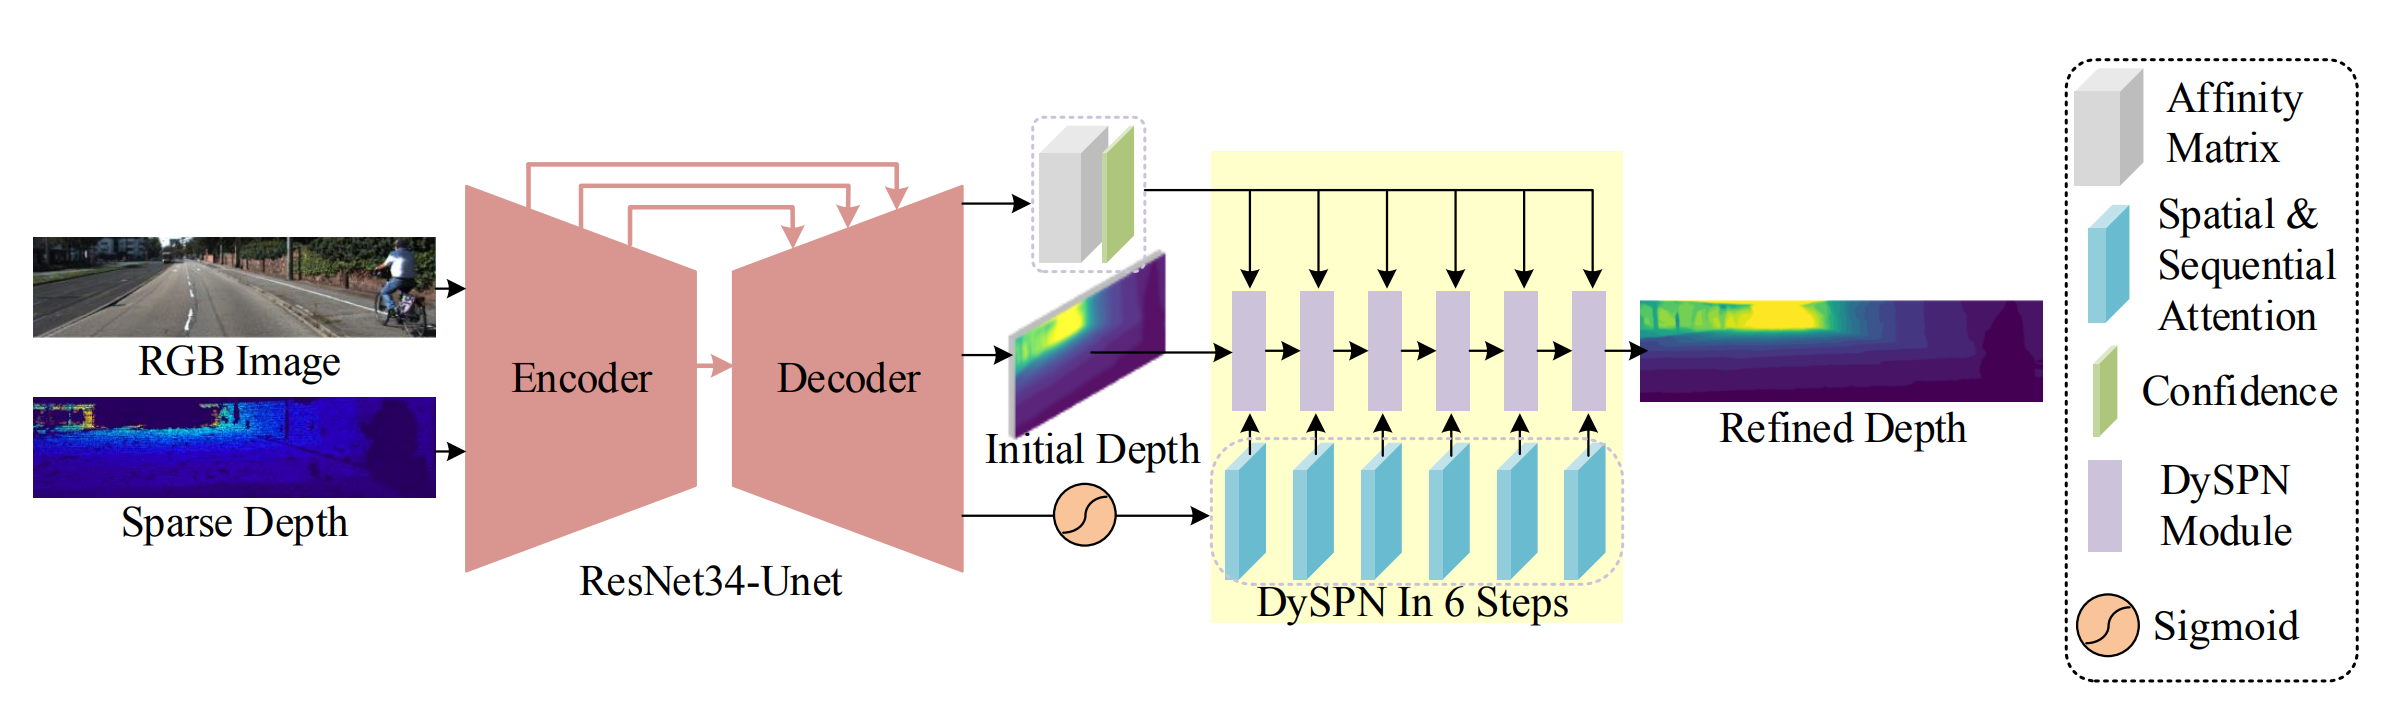
\includegraphics[width=\textwidth]{figures/dyspn.png}
    \caption{DySPN Architecture}
    \label{fig:dyspn_architecture}
\end{figure}

We chose DySPN for several key reasons, as summarized in Table~\ref{table:dyspn_reasons}.

\begin{table}[h!]
\centering
\begin{tabular}{@{}p{4.5cm}p{9.3cm}@{}}
\toprule
\textbf{Reason} & \textbf{Description} \\
\midrule
Real-time Performance & The network can achieve inference in 38ms, making it suitable for teleoperation applications. \\
\midrule
Benchmark Performance & DySPN achieves state-of-the-art results on the KITTI depth completion benchmark with an RMSE of 709.12mm. \\
\midrule
Supervised Learning  & While supervised learning typically requires extensive ground truth data, our simulation-based development environment using CARLA provides precise depth information for training. \\
\bottomrule
\end{tabular}
\caption{Key Reasons for Selecting DySPN Architecture}
\label{table:dyspn_reasons}
\end{table}

The ability to use CARLA's precise depth camera for generating ground truth data makes this supervised approach particularly attractive. The network's architecture, which decouples neighborhood relationships based on distance and uses attention mechanisms to dynamically adjust affinities, aligns well with our goal of creating accurate depth reconstructions for teleoperation interfaces.
For our implementation, we made several modifications to adapt the network to our specific requirements. First, we adjusted the network architecture to accommodate our image resolution of 1280x720, compared to the original KITTI resolution. Second, we reimplemented certain operations to ensure compatibility with PyTorch's JIT compilation, enabling seamless deployment in our C++ production environment.

\subsection{W-Shaped Development Cycle}
The development approach for our depth completion model aligns with the W-shaped development cycle for learning assurance, as proposed by the European Union Aviation Safety Agency (EASA) \cite{easa2024}. This cycle provides a structured framework for developing \ac{AI} based systems.
Similar to the V-model \cite{vmodel} that is widely used for software development for safety related products, W-Shaped Development Cycle introduce a second development point for the development of the \ac{AI} model.
We have adapted our proof-of-concept level project to follow this method, which can be mapped to the key stages of the W-shaped cycle as shown in the Figure \ref{table:wshaped_cycle}.

\begin{table}[h!]
    \centering
    \begin{tabular}{@{}p{1cm}p{13cm}@{}}
    \toprule
    \textbf{\#} & \textbf{Stage Description} \\
    \midrule
    1 & \textbf{Requirements Management:} We derived clear requirements from our literature review and identified research gaps, guiding the development of both the depth completion model and the overall interface. \\
    \midrule
    2 & \textbf{Data Management \& Verification:} We selected appropriate sensor configurations, including a 120-degree FOV camera and 1280x720 resolution at 30 fps. We utilized simulation data from CARLA for development and testing. \\
    \midrule
    3 & \textbf{Learning Process Management:} We made decisions regarding the training algorithm and architecture for depth completion, selected performance evaluation metrics (e.g., iRMSE, iMAE), and chose appropriate hardware and software frameworks for implementation. \\
    \midrule
    4 & \textbf{Model Training:} This phase involved the actual training of our depth completion model, separate from the main interface development. \\
    \midrule
    5 & \textbf{Learning Process Verification:} While not conducting extensive tests at this stage, we verified the learning process by evaluating the trained model's performance on test cases and iterating on the model design as needed. \\
    \midrule
    6 & \textbf{Model Implementation:} We implemented the trained depth completion model within the Integrated View interface and optimized it for real-time performance in the teleoperation context. \\
    \midrule
    7 & \textbf{Inference Model Verification:} We ensured the implemented model behaved consistently with the trained model and verified real-time performance within the interface. \\
    \bottomrule
    \end{tabular}
    \caption{Explanation of the W-shaped development cycle stages and their application to our depth completion model development}
    \label{table:wshaped_cycle}
    \end{table}

By framing our development approach within this W-shaped cycle, we demonstrate adherence to a structured methodology for developing \ac{AI}-based systems, even at a proof-of-concept level. This approach ensures consideration of key stages in \ac{AI} system development and aligns with industry best practices for learning assurance.

\subsection{Simulation Setup}

Our simulation environment integrates CARLA simulator with Autoware autonomous driving stack through the CARLA-Autoware Bridge \cite{carla_aw_bridge24}. This setup enables us to create a controlled testing environment for our visualization approaches while maintaining realistic driving scenarios.


\subsubsection{Vehicle and Sensor Configuration}
The sensor configuration aims to replicate TUM's EDGAR vehicle while maintaining computational efficiency in the simulation environment. The primary sensors are detailed in Table~\ref{table:sensor_configuration}.

\begin{table}[h!]
\centering
\begin{tabular}{@{}p{4cm}p{10cm}@{}}
\toprule
\textbf{Sensor Type} & \textbf{Specifications/Details} \\
\midrule
Frontal LiDARs & Two LiDARs with 120-meter range, positioned at the front left and right corners with 45-degree angles. \\
\midrule
LiDAR Specifications &
20 Hz rotation rate \par
1,310,720 points per second \par
64 channels \\
\midrule
Front-facing Camera & Resolution: 1280x720, Field of View (FOV): 120°. \\
\midrule
Depth Camera & Matches the specifications of the front-facing camera. \\
\midrule
GNSS and IMU Sensors & Provides localization and orientation data. \\
\bottomrule
\end{tabular}
\caption{Sensor Configuration for Vehicle Simulation}
\label{table:sensor_configuration}
\end{table}

\subsubsection{Environment Selection}
Initial development and data collection were conducted in CARLA's Town10 environment. However, as our target user group consists of German operators, we identified potential limitations in using U.S.-based road layouts for situational awareness evaluation. To address this, we developed a custom map based on a real location in Munich, Germany. This ensures that the traffic scenarios and road layouts are familiar to our test subjects, providing more relevant data for evaluating operator performance. The details of the custom map development are discussed in Section \ref{section:mapcreationforcarla}.
\subsection{Data Collection}


To train our depth completion network, we developed a ROS application that collects synchronized sensor data from the CARLA simulation environment. The application subscribes to three main data streams: LiDAR point clouds, camera images, and depth camera outputs (which serve as ground truth). The data collection setup is illustrated in Figure \ref{fig:data_collection}.
We gathered a dataset of ${\sim}10,000$ images by manually driving through the simulation environment with dynamic weather conditions enabled. To ensure diversity in the collected data, our collection script captured sensor data at random time intervals. This approach helps prevent oversampling of similar scenes and ensures a more representative dataset.
The preprocessing pipeline transforms point cloud data into camera space using the sensor extrinsic parameters, normalizes depth values to 8-bit range (0-255) for efficient storage, and projects 3D points onto the image plane using camera intrinsics. The processed data was stored in NumPy's .npy format using 32-bit floating-point precision per pixel. This format was chosen for its efficient storage and fast loading capabilities during training, while maintaining sufficient numerical precision for depth values. The pint cloud input can be seen in Figure \ref{fig:pointcloud_input}
\begin{figure}[h]
    \centering
    \begin{subfigure}{\textwidth}
        \centering
        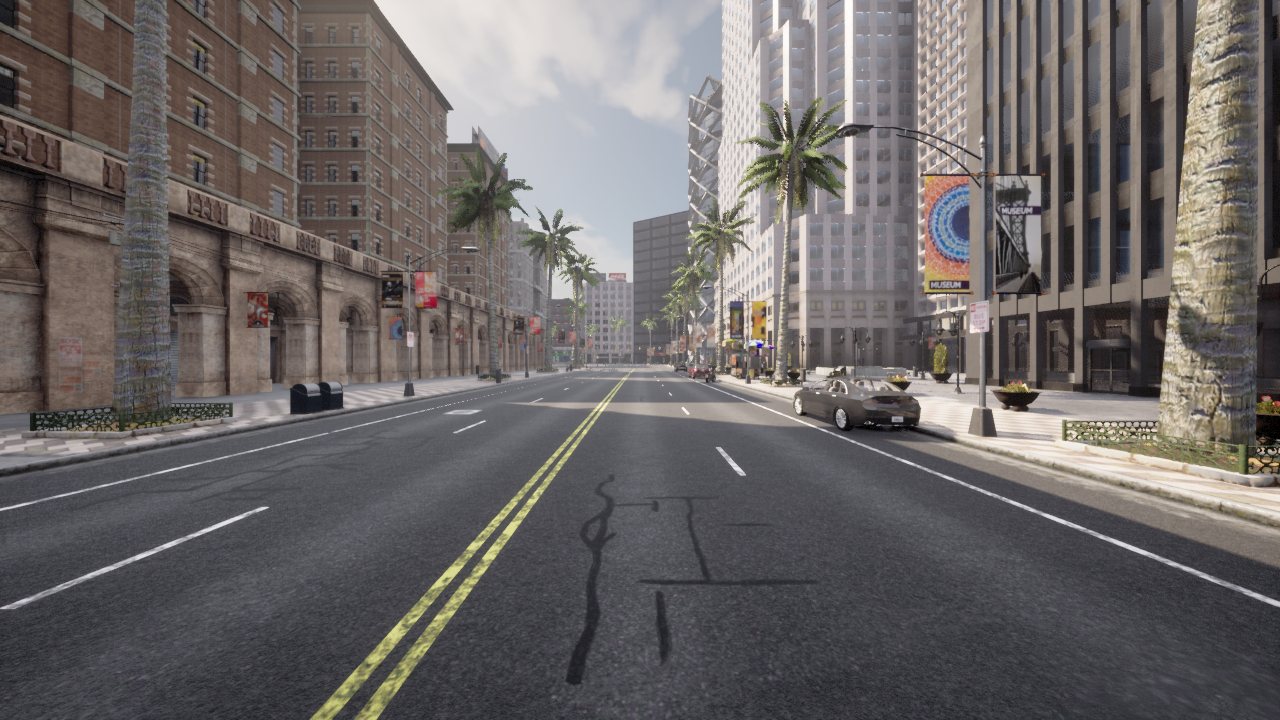
\includegraphics[width=\textwidth, trim=0 200pt 0 200pt, clip]{figures/rgb.png}
        \caption{RGB camera image from CARLA simulation}
        \label{fig:rgb_input}
    \end{subfigure}
    \begin{subfigure}{\textwidth}
        \centering
        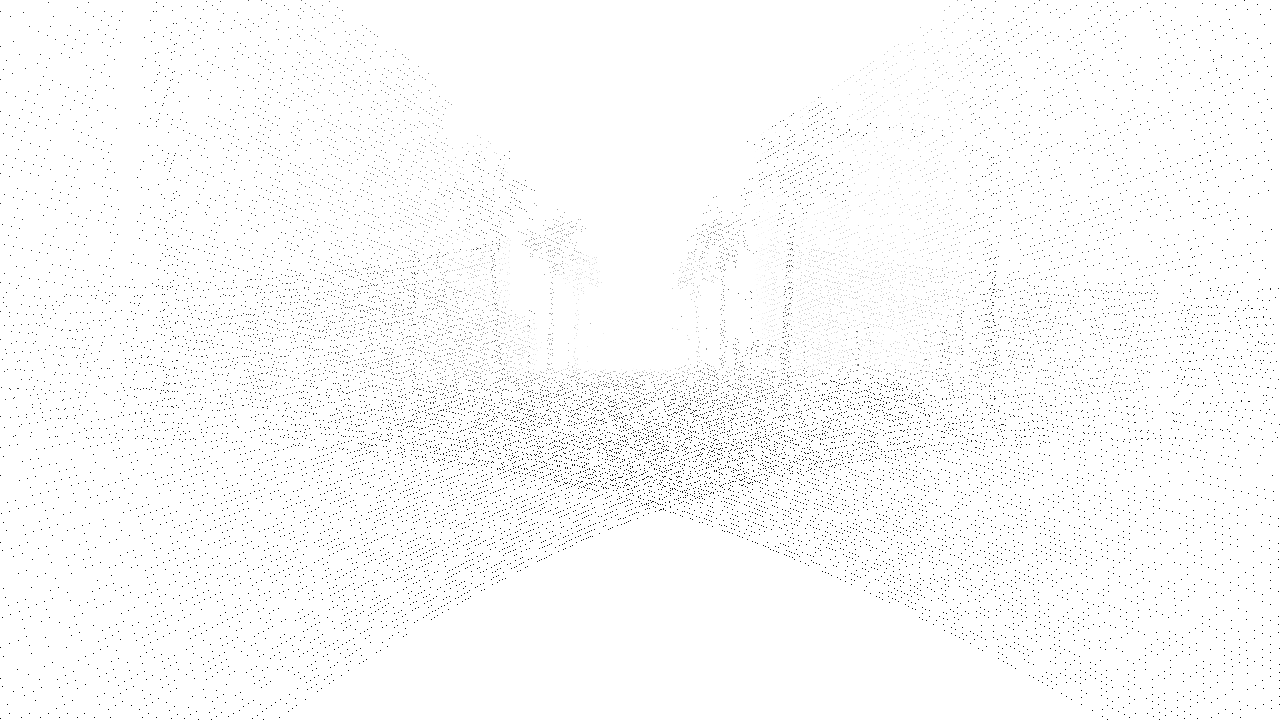
\includegraphics[width=\textwidth, trim=0 200pt 0 200pt, clip]{figures/point_cloud.png}
        \caption{Projected LiDAR point cloud showing sparse depth information}
        \label{fig:pointcloud_input}
    \end{subfigure}
    \begin{subfigure}{\textwidth}
        \centering
        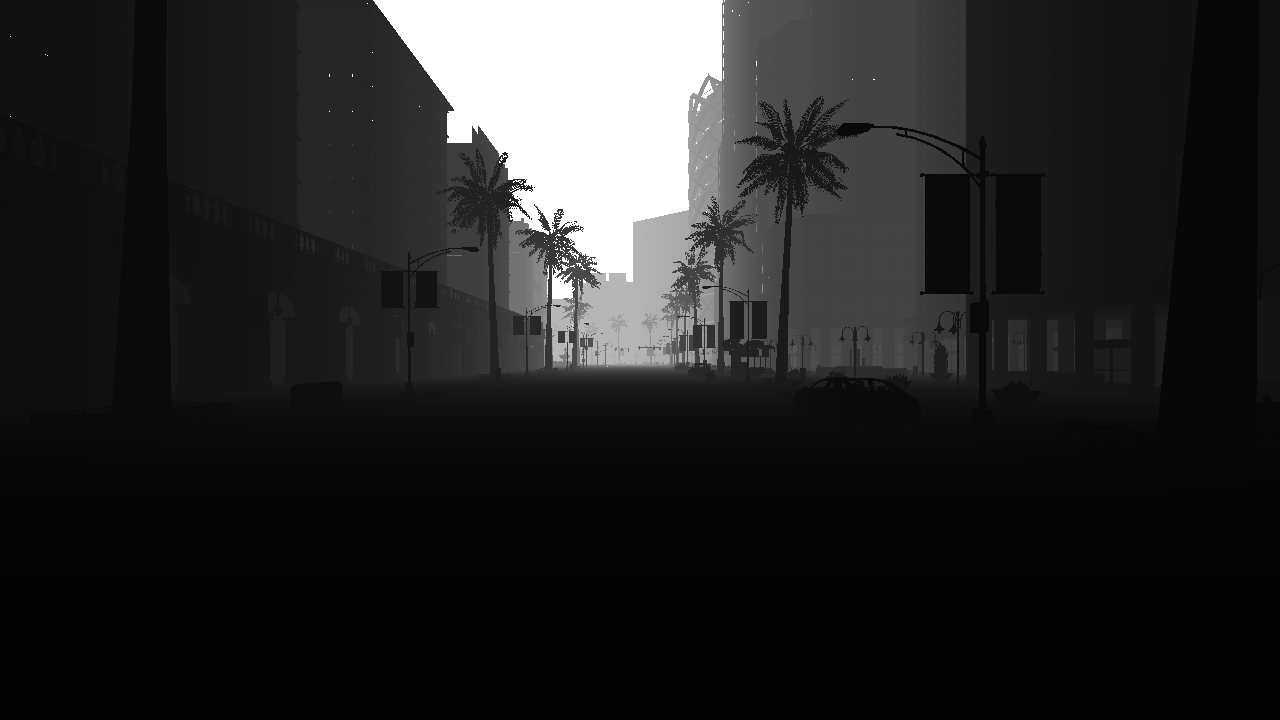
\includegraphics[width=\textwidth, trim=0 200pt 0 200pt, clip]{figures/depth_gt.png}
        \caption{Ground truth depth map from CARLA's depth camera}
        \label{fig:depth_gt}
    \end{subfigure}
    \caption{Example of collected training data showing the three input types: RGB image, sparse LiDAR point cloud, and ground truth depth map}
    \label{fig:data_collection}
\end{figure}
\FloatBarrier

\subsection{Training}

We conducted the training on an NVIDIA RTX 4090 GPU using the AdamW optimizer, which combines the benefits of the Adam optimizer with weight decay regularization. AdamW addresses the potential interference between L2 regularization and momentum in the original Adam optimizer, making it particularly effective for \ac{DL} tasks by providing better generalization and more stable training dynamics.

Through grid search optimization, we evaluated learning rates ranging from 0.01 to 0.0001 and batch sizes of 1 and 2, with hardware limitations preventing larger batch sizes. The initial five epochs of each configuration were analyzed to assess training stability and validation loss trends. Based on these results, we selected a learning rate of 0.001 and a batch size 1 for the final training run of 100 epochs. We implemented a learning rate scheduler that reduces the learning rate when the validation loss plateaus to optimize the training process.

\begin{figure}[h]
    \centering
    \begin{subfigure}{0.48\textwidth}
        \centering
        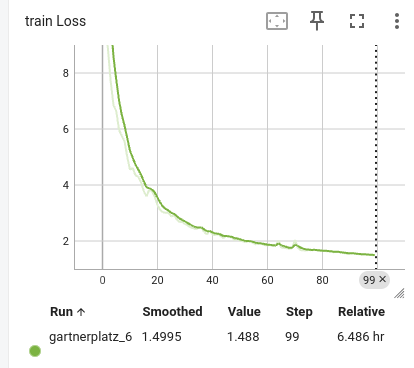
\includegraphics[width=\textwidth]{figures/train.png}
        \caption{Training loss curve}
        \label{fig:train_curve}
    \end{subfigure}
    \hfill
    \begin{subfigure}{0.48\textwidth}
        \centering
        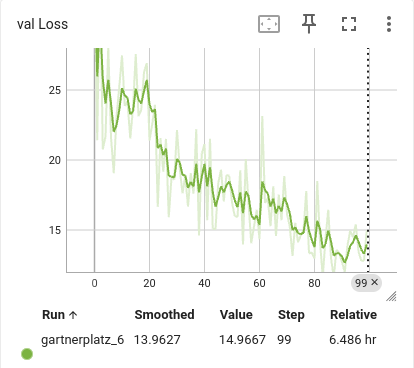
\includegraphics[width=\textwidth]{figures/validation.png}
        \caption{Validation loss curve}
        \label{fig:val_curve}
    \end{subfigure}
    \caption{Training and validation loss curves over 100 epochs}
    \label{fig:training_curves}

\end{figure}
The loss function combines three components:


\[
L_{total} = \alpha L_1 + \beta L_2 + \gamma L_{SSIM}
\]


where the Structural Similarity Index Measure (SSIM) loss evaluates the perceptual quality between predicted and ground truth depth maps. SSIM considers luminance, contrast, and structural information, making it particularly effective for maintaining overall depth map consistency. The L1 and L2 losses were specifically weighted to focus on depths below 120 meters, aligning with our LiDAR's range:

\[
    L_{1,2} = \begin{cases}
    L_{1,2}(pred, gt) & \text{if } depth < 120m \\
    0 & \text{otherwise}
    \end{cases}
\]

The validation loss shows consistent improvement throughout training, decreasing from approximately 30 to 15 over 99 epochs. While there are noticeable oscillations in the validation curve, particularly in earlier epochs, the overall downward trend indicates successful model convergence. The final validation loss of 14.96 and smoothed curve suggest that the learning rate scheduler effectively managed the training process.


\begin{figure}[h]
    \centering
    \begin{subfigure}{\textwidth}
        \centering
        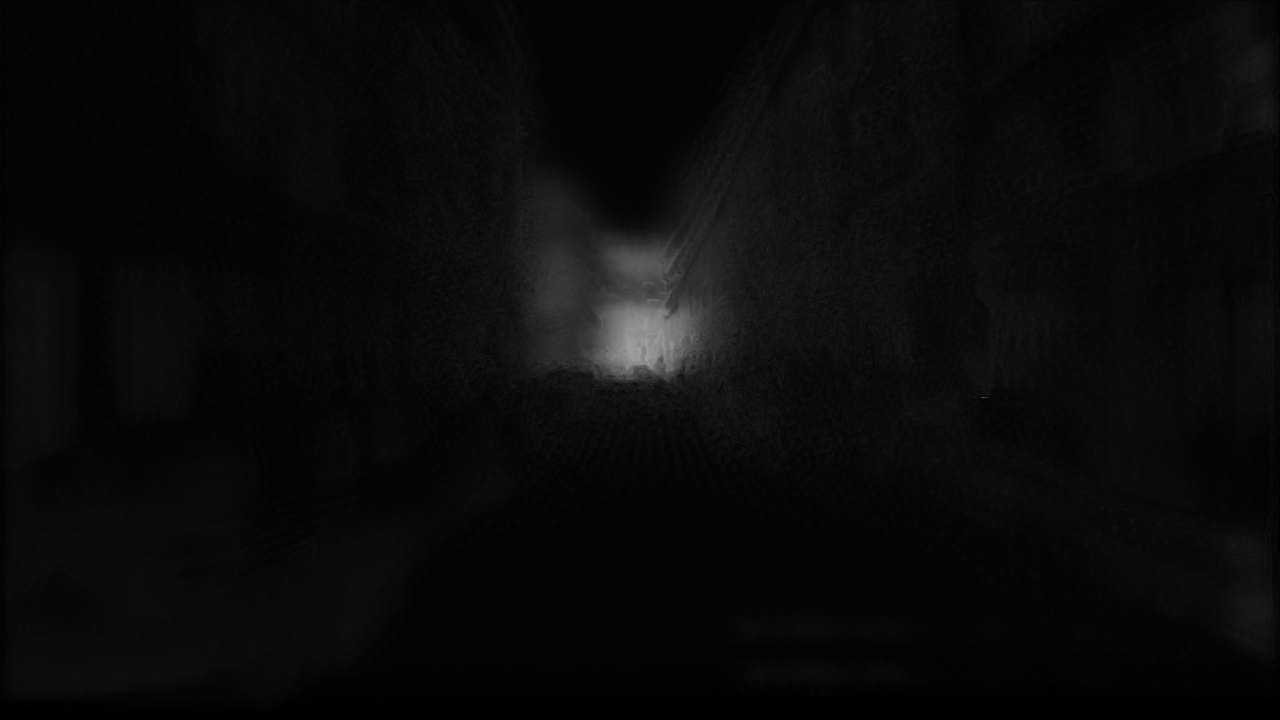
\includegraphics[width=\textwidth, trim=0 200pt 0 200pt, clip]{figures/step1.png}
        \caption{Epoch 1}
        \label{fig:epoch1}
    \end{subfigure}
    \hfill
    \begin{subfigure}{\textwidth}
        \centering
        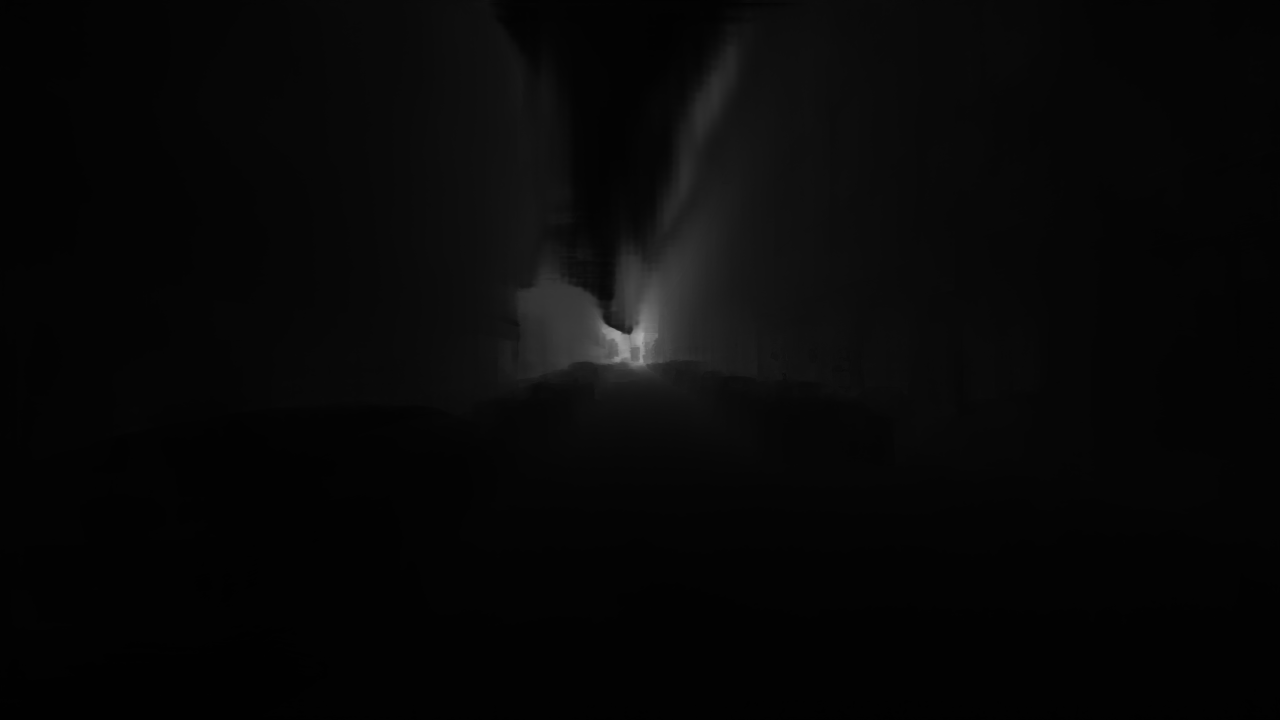
\includegraphics[width=\textwidth, trim=0 200pt 0 200pt, clip]{figures/step38.png}
        \caption{Epoch 38}
        \label{fig:epoch38}
    \end{subfigure}
    \hfill
    \begin{subfigure}{\textwidth}
        \centering
        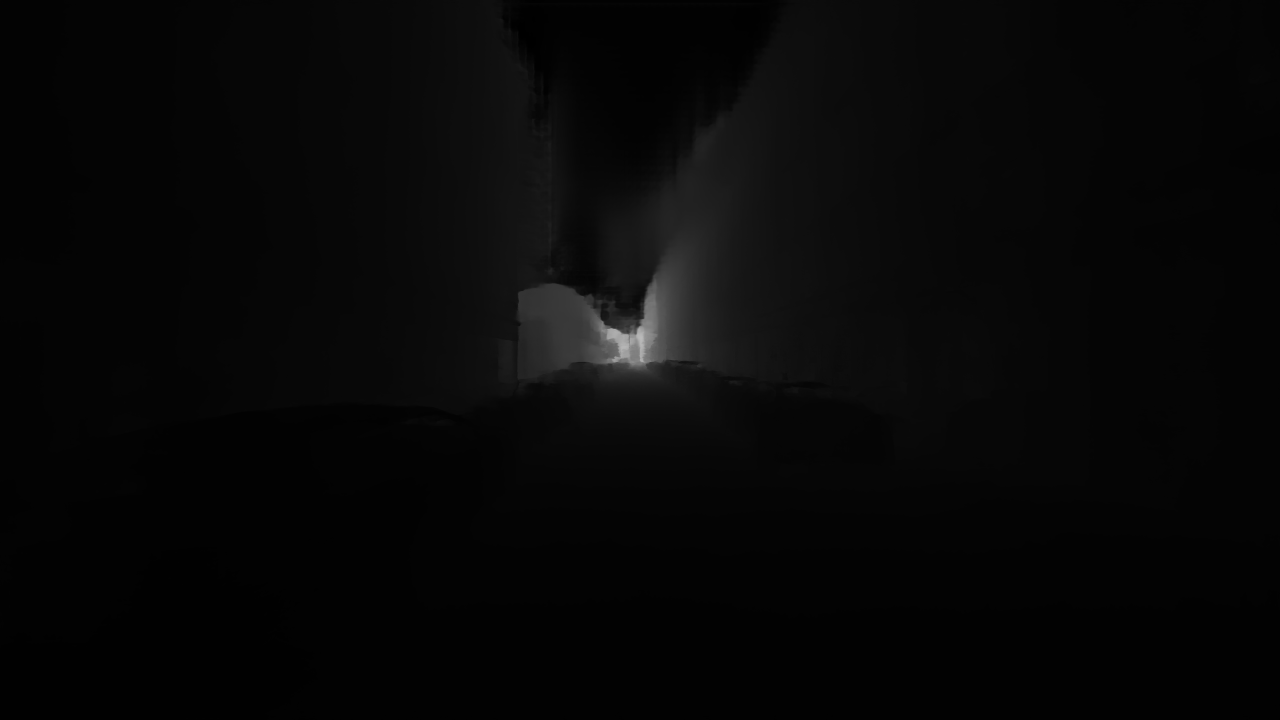
\includegraphics[width=\textwidth, trim=0 200pt 0 200pt, clip]{figures/step99.png}
        \caption{Epoch 99}
        \label{fig:epoch99}
    \end{subfigure}
    \caption{Evolution of depth completion output during training}
    \label{fig:training_progress}
\end{figure}

The sample outputs in Figure \ref{fig:training_progress} demonstrate the model's learning progression through epochs 1, 38, and 99, showing increasingly refined depth estimation and improved preservation of structural details. The final output at epoch 99 exhibits smooth depth transitions and accurate depth completion, indicating successful training despite the oscillations in the validation curve.
\begin{figure}
    \centering
    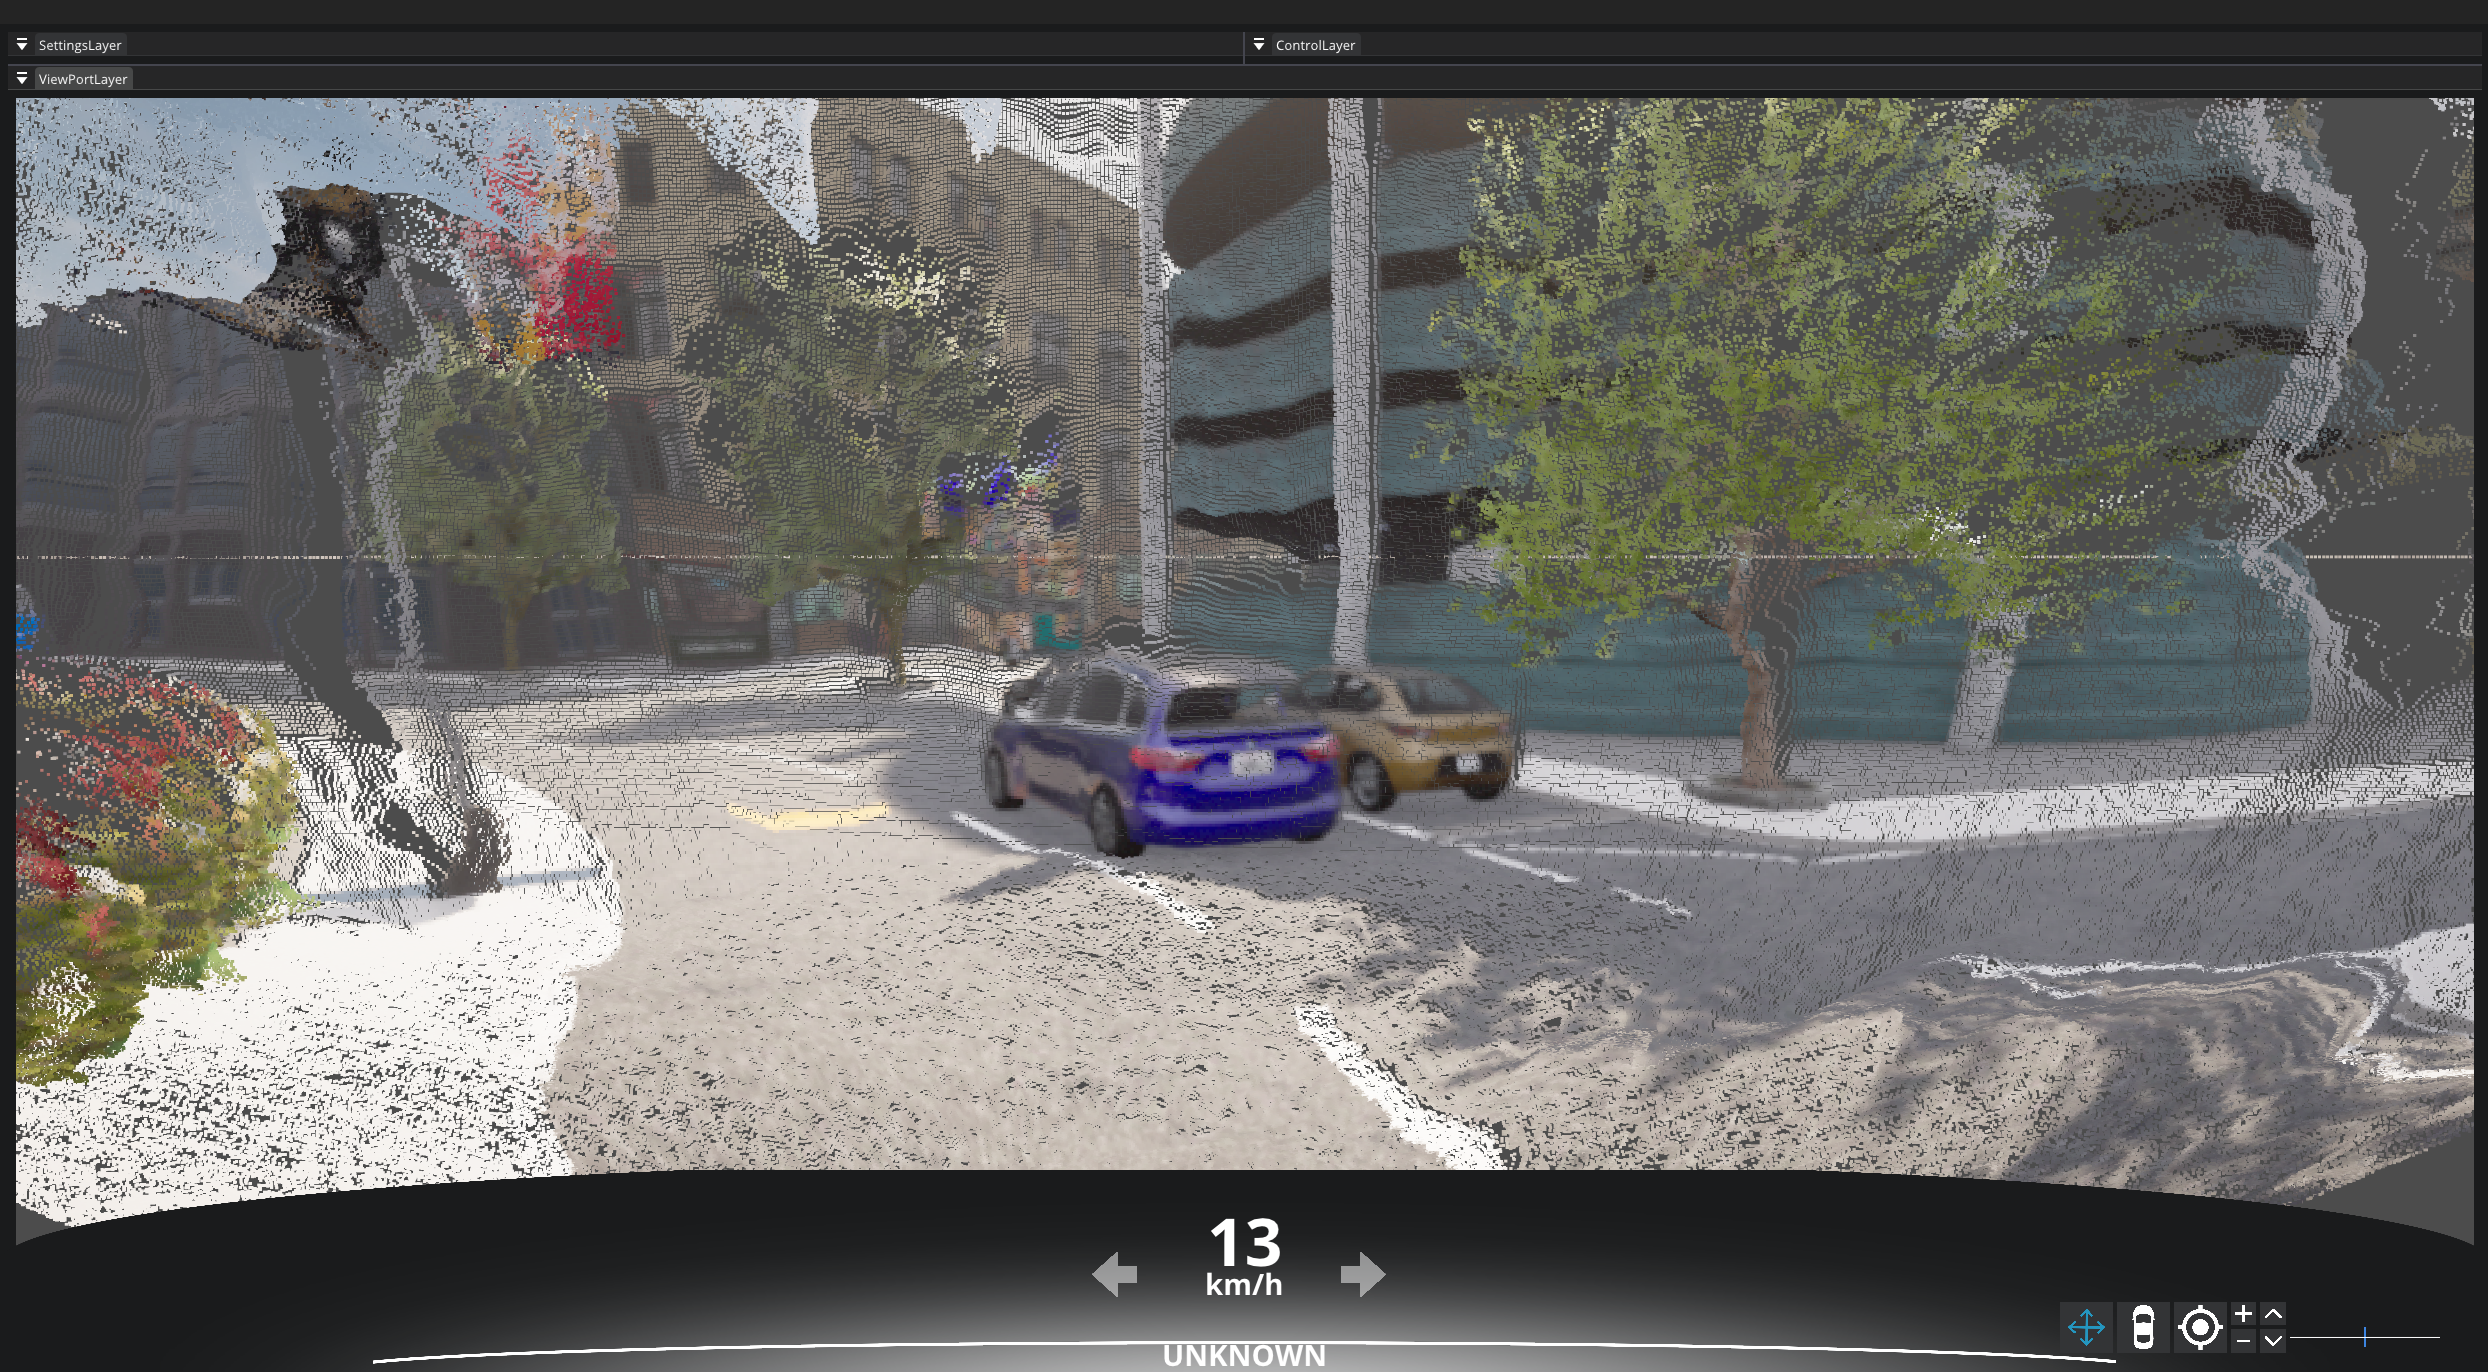
\includegraphics[width=\textwidth, trim=0 150pt 0 50pt, clip]{figures/depth_comp.png}
    \caption{The point cloud generated by the output from the depth completion model}
    \label{fig:depth_completion_result}
\end{figure}

\section{Performance Optimization}

For a teleoperation system to be effective, real-time performance is crucial. Research indicates that system latency should be kept below 300ms for controlled driving, and frame rates should be maintained above 5 Hz to avoid significant performance degradation \cite{neumeier2023feasibility}. Our optimization efforts focus on two main aspects: operator interface performance and network performance.

\subsubsection{Operator Interface Performance}
Our system runs on high-performance hardware, utilizing an NVIDIA RTX 4090 GPU and the latest generation Intel Core i9 processor. Despite this powerful configuration, there are several computational bottlenecks required optimization.

The depth completion model represents our most significant performance bottleneck, requiring 60-70ms per frame for estimation. At this processing speed, the system would be limited to less than 15 fps if processed synchronously. To overcome this limitation, we implemented an asynchronous processing approach where the depth estimation runs on a parallel thread. This allows visual updates to occur at full frame rate while depth information updates at a lower frequency. The difference in update rates is barely noticeable to operators due to the smooth integration of the parallel processing.

The next significant CPU bottleneck involves processing and rendering point cloud data. We addressed this using the PCL library, implementing efficient filtering and concatenation of LiDAR inputs. Points that are too close to each other are filtered out to maintain rendering performance while preserving visual quality.

\subsubsection{Network Performance}
Network performance is critical for teleoperation systems, as they must operate within mobile network constraints. Our optimization strategy focuses on minimizing data throughput while maintaining essential information transmission.
We carefully select which data to transmit from vehicle to interface:
\begin{itemize}
\item RGB camera feed (1280x720 resolution)
\item Subset of point cloud data for frontal view
\item Regulatory elements and perception outputs
\end{itemize}
Instead of transmitting full depth images, we send point cloud data in a compressed format. This approach is more efficient as the sparse point cloud contains significant empty space, and point cloud reconstruction occurs on the operator side. Additionally, only relevant points for the frontal view are transmitted, further reducing bandwidth requirements.
Through these optimizations, we maintain real-time performance while working within network bandwidth constraints, ensuring effective teleoperation capability.